\documentclass[numbers=noenddot,12pt,a4paper]{scrartcl}
\usepackage[greek,ngerman]{babel}
\usepackage[T1]{fontenc}
\usepackage[utf8]{inputenc}
\usepackage{fullpage}
\usepackage{libertine}
\usepackage{ziffer}
\usepackage{graphicx}
\usepackage{units}
\usepackage[infoshow]{tabularx}
\usepackage{amsmath}
\usepackage{amssymb}
\usepackage{wrapfig}
\usepackage{esint}
\usepackage{float}
\usepackage{wrapfig}
\usepackage[font=small]{caption}
\usepackage{subcaption}
\usepackage{lscape}
\usepackage{hyperref}

\renewcommand{\thefigure}{Abb. \arabic{figure}}

\captionsetup[wrapfigure]{name=}
\captionsetup[figure]{name=}
\newcommand{\degree}{^\circ}
\newcommand{\diff}{\textnormal{d}}
\newcommand{\tenpo}[1]{\cdot 10^{#1}}
\newcommand{\greek}[1]{\greektext#1\latintext}
\newcommand{\ix}[1]{_\text{#1}}
\newcommand{\imag}{\mathbf{i}}
\newcommand{\tilt}[1]{\textit{#1}}
\newcommand{\grad}[1]{\textit{grad}\left(#1\right)}
\newcommand{\divergenz}[1]{\textit{div}\left(#1\right)}
\newcommand{\euler}{\mathnormal{e}}
\newcommand{\fett}[1]{\textbf{#1}}

\title{Protokoll: Hall-Effekt in Halbleitern}
\author{\underline{Tom Kranz}, Philipp Hacker}
\date{\today}

\begin{document}
%\setcounter{page}{2}
%\setcounter{section}{1}
\maketitle
\begin{center}
Betreuer: M. von der Ehe\\
Versuchsdatum: 18.11.2014\\
\begin{table}[h]
\centering
Note: %TODO Gute Note erhalten :)
\begin{tabularx}{1.5cm}{|X|}
\hline \\ \\
\hline
\end{tabularx}
\end{table}
\end{center}
\vspace*{\fill}
\tableofcontents
\vfill
\newpage
\section{Motivation}
Halbleiter sind wichtige Rohstoffe für die moderne Elektronik -- aufgrund ihrer leicht und über viele Größenordnungen hinweg anpassbaren, besonderen elektrischen Eigenschaften finden sie Verwendung in vielen sogenannten aktiven Bauteilen, die nicht nur Effekte der Leitung von Strom ausnutzen, sondern die Stromleitung auf komplexe Weise auch selbst steuern können. Ausschlaggebend für ihre Funktion sind Kenngrößen von Halbleitern wie die Anzahldichten $n$ beziehungsweise $p$ und die Beweglichkeiten $\mu_n$ beziehungsweise $\mu_p$ der freien Ladungsträger und die Bandlücke $E\ix{G}$. Die Messung dieser Größen mittels des Hall-Effekts soll Gegenstand dieses Versuchs sein.
\section{Grundlagen}
\subsection{Halbleiter}
Das Bandmodell weist alle Elektronen eines Festkörpers energetisch sogenannten Bändern zu; Bereichen des Energieniveauschemas, in denen die quantenmechanisch erlaubten Energieniveaus so dicht beeinander liegen, dass man sie innerhalb der Bänder gut durch ein Kontinuumsspektrum nähern kann. Diese Bänder können entweder durch sogenannte Energielücken getrennt sein oder überlappen -- dies bestimmt die grundlegenden elektrischen Eigenschaften des Festkörpers. Da die Elektronen in solchen Systemen nur dann einen Strom bilden können, wenn die verfügbaren Energiebänder nicht entweder völlig belegt oder völlig besetzt sind und weil Energieniveaus im Groben von niedrig- nach hochenergetisch besetzt werden, spricht man bei Festkörpern mit überlappenden Energiebändern, die zwangsweise jeweils nur zu einem Teil belegt sein können, von elektrischen Leitern und bei Festkörpern mit Energielücke zwischen dem letzten belegten und dem ersten unbelegten Band von Isolatoren, da das niedergelegene Band mit den Elektronen des Systems völlig belegt ist und das höhergelegene Band keine Elektronen beinhaltet.\\
Ist die Energielücke jedoch so klein, dass die Fermiverteilung, die ja die Zustands-/Energie\-verteilung von Fermionen wie dem Elektron bestimmt, im Bereich der Energielücke bei Arbeitstemperatur eine merkliche Aufweichung der Besetzungsverteilung vorhersagt, spricht man von Halbleitern. Typische Größen für Bandlücken von Halbleitern liegen im Bereich weniger Elektronenvolt, so hat Silicium (bei Raumtemperatur) eine Bandlücke von $\unit[1,12]{eV}$, Germanium sogar nur $\unit[0,67]{eV}$.
\subsubsection{Kenngrößen von Halbleitern}
Wichtig für ein elektronisches Bauteil ist natürlich dessen elektrische Leitfähigkeit $\sigma$. Bei Halbleitern hängt diese von der Anzahldichte ins Leitungsband übergegangener Elektronen $n$ und ihrer Beweglichkeit $\mu_n$ und der Anzahldichte der im Valenzband nicht besetzten Zustände, den Defektelektronen oder einfach "`Löchern"', $p$ und ihrer Beweglichkeit $\mu_p$ ab:
\begin{align}
\sigma=e\cdot\left(n\cdot\mu_n+p\cdot\mu_p\right)
\end{align}
%TODO Warum Boltzmann-Verteilung für intrinsische Ladungsdichte?
%TODO Herleitung E_G aus ln(σ_i)(1/T)
\subsubsection{Dotierung}
%TODO Reserve, Erschöpfung, intrinsischer Bereich erläutern
\subsection{Hall-Effekt}
\subsubsection{Nutzen für Halbleitertechnik}
%TODO Hall-Konstante aus n, p Ladungsträgern und μ_n, μ_p herleiten
\section{Auswertung}
\subsection{Undotierter Ge-Kristall}
Zuerst sollte die Leitfähigkeit des undotierten Germaniums in Abhängigkeit von der Temperatur bestimmt werden. Dafür haben wir eine Stromquelle an die Kontakte des Kristalls angeschlossen und die über dem Kristall abfallende Spannung und den Stromfluss gemessen. Wir haben dafür eine spannungsrichtige Schaltung der Messgeräte gewählt. Daraus erhalten wir die Leitfähigkeit über die Beziehung:
\begin{align}
\vec{j}&=\sigma\cdot\vec{E}&\left|\cdot h\cdot t\cdot b\cdot \vec{e}_I\right.\nonumber\\
\vec{j}\cdot h\cdot t\cdot b\cdot\vec{e}_I=I\cdot b&=\sigma\cdot h\cdot t\cdot\vec{E}\cdot b\cdot \vec{e}_I=\sigma\cdot U\cdot h\cdot t &\left|:(U\cdot h\cdot t)\right.\\
\frac{I\cdot b}{U\cdot h\cdot t}&=\sigma
\end{align}
Mit der Höhe $h$, der Breite $b$ (entlang der Stromrichtung $\vec{e}_I$) und der Tiefe $t$ des Kristalls. Wegen den Überlegungen hinter Gleichung \ref{eq:logsigma} bietet sich der lineare Fit der $\ln\left(\sigma\right)$-$\frac{1}{T}$-Beziehung an, der in \ref{img:undlogsig} dargestellt ist, um die Bandlücke $E\ix{G}$ des Germaniums zu bestimmen.
\begin{figure}[H]
	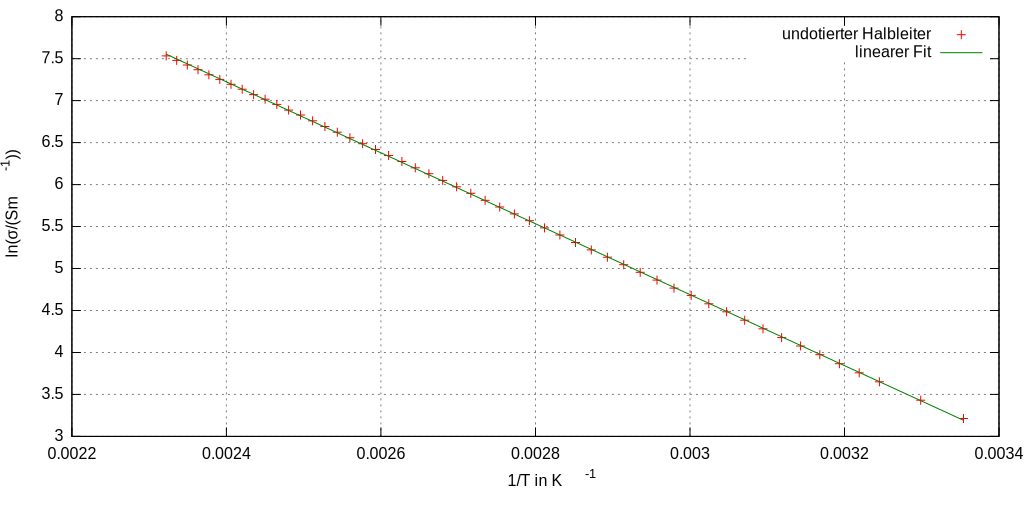
\includegraphics[width=\textwidth]{messwerte/undotiert.pdf}
	\caption{$\ln\left(\unit[\sigma]{/Sm^{-1}} \right)$ über $\frac{1}{T}$ Diagramm mit Fit zur Funktion $f\left(\frac{1}{T}\right)=a\cdot\frac{1}{T}+b$} \label{img:undlogsig}
\end{figure}
Dabei hat sich mittels Methode der kleinsten Quadrate eine Steigung von $a=\unit[-4225,73\,(403)]{K}$ ergeben. Nach Gleichung \ref{eq:logsigma} ist dies $-\frac{E\ix{G}}{2\cdot k\ix{B}}$, also $E\ix{G}=-2\cdot k\ix{B}\cdot a=\unit[0,72828\,(69)]{eV}$.
\subsection{Dotierte Ge-Kristalle}
\subsubsection{Ladungsträgerdichte bei Raumtemperatur}
Als nächstes wurde die Hall-Spannung $U\ix{H}$ in einem p- und einem n-dotierten Germanium-Kristall als Funktion des angelegten Magnetfelds $B$ gemessen, um die Hall-Konstante und daraus die Ladungsträgerkonzentration nach \ref{eq:hall-konst}, beziehungsweise einer Näherung dieser Beziehung, zu bestimmen. In \ref{img:hall-konst} ist $U\ix{H}$ über $B$ aufgetragen und an eine Funktion $U(B)=R\ix{H}\cdot B$ angepasst.
\begin{figure}[H]
	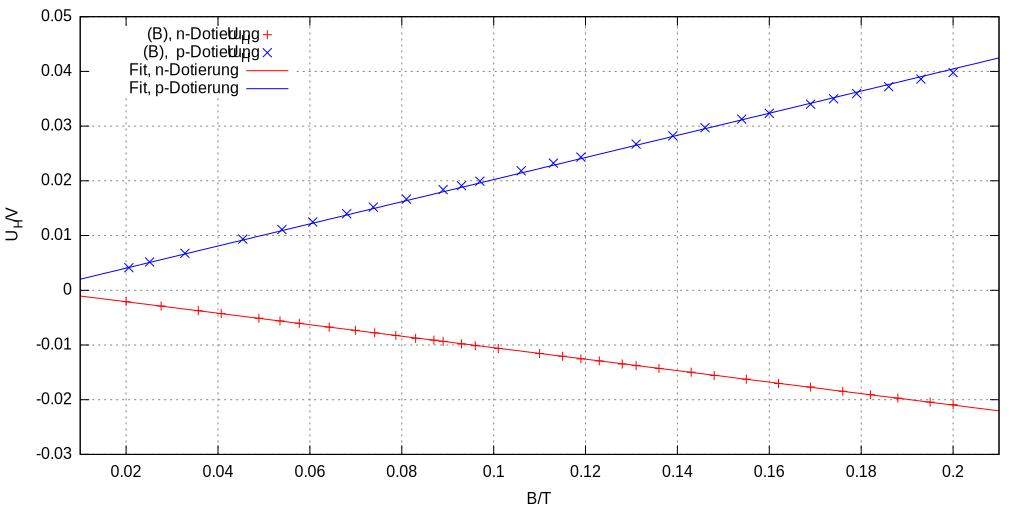
\includegraphics[width=\textwidth]{messwerte/hallkonstanten.pdf}
	\caption{$U\ix{H}$ über $B$ Diagramm mit Fit zur Funktion $U(B)=R\ix{H}\cdot B$} \label{img:hall-konst}
\end{figure}
Dabei hat sich ein Anstieg von $R\ix{H}=\unit[-0,104947\,(46)]{VT^{-1}}$ für die n-dotierte und $R\ix{H}=\unit[0,202243\,(461)]{VT^{-1}}$ für die p-dotierte Probe ergeben.
\subsubsection{Temperaturabhängigkeit der Ladungsträgerdichten}
Nun wurde bei festem Magnetfeld $B$ und Querstrom $I$ die Temperatur der Kristalle variiert, um die Veränderung der Hall-Spannung und damit der Hallkonstante und schließlich der Ladungsträgerkonzentration zu beurteilen. Nach \ref{ch:dot} erwartet man im hohen Temperaturbereich einen Verlauf $\propto \exp\left(-\frac{E\ix{G}}{2\cdot k\ix{B}\cdot T} \right)$, im mittleren Temperaturbereich einen konstanten Verlauf und im niedrigeren Temperaturbereich einen Verlauf $\propto \exp\left(-\frac{E\ix{d}}{2\cdot k\ix{B}\cdot T} \right)$, was sich in der logarithmischen Darstellung von $n$ beziehungsweise $p$ über $\frac{1}{T}$ bemerkbar machen sollte. Diese ist in \ref{img:dotierttemperatur} zu sehen. Tatsächlich sieht man im Bereiche höherer Temperatur einen annähernd linear fallenden Verlauf, der bei niedrigerer Temperatur in ein Plateau über geht. Dies sind jeweils die Bereiche, in denen intrinsische Leitung, beziehungsweise Störstellenerschöpfung auftritt. Die Störstellenreserve lässt sich in unserem Temperaturbereich noch nicht feststellen, da unsere niedrigste Temperatur gerade einmal $\unit[294,85]{K}$ betrug. Jedoch sind die Anstiege in der logarithmischen Darstellung unterschiedlich; man würde erwarten, dass in der intrinsischen Leitung, deren einziger Parameter die Halbleitermaterial-Konstante $E\ix{G}$ ist, bei gleichen Halbleiterrohstoffen gleiche Anstiege zu sehen sind.
\begin{figure}[H]
	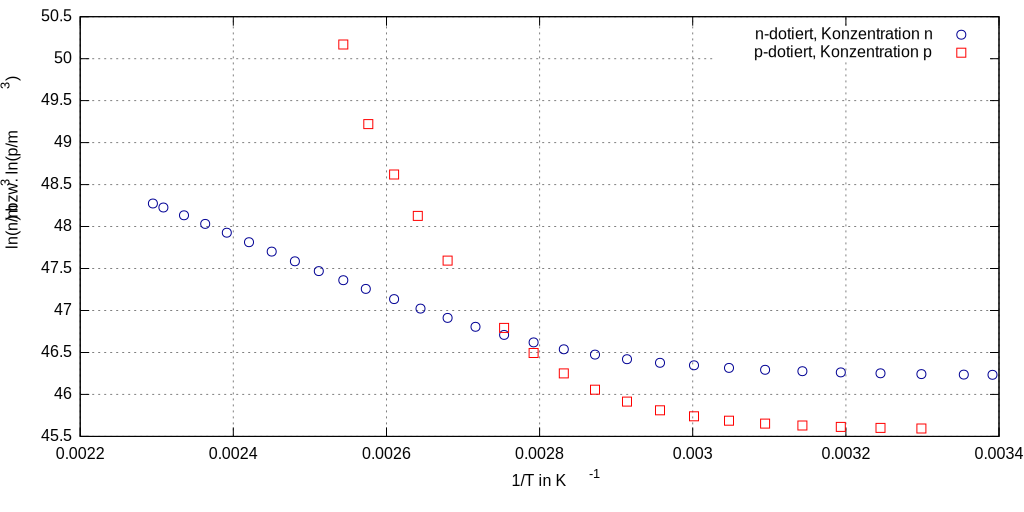
\includegraphics[width=\textwidth]{messwerte/temperaturkonzentration.pdf}
	\caption{$\ln\left(\unit[n]{\cdot m^3}\right)$ über $\frac{1}{T}$ Diagramm} \label{img:dotierttemperatur}
\end{figure}
\subsubsection{Temperaturabhängigkeit der Ladungsträgerbeweglichkeiten}
Wie in \ref{ch:beweg} bereits erläutert und in \ref{img:beweglichkeit} zu sehen, wird die Beweglichkeit der Ladungsträger durch, hauptsächlich 2 Umstände eingeschränkt: Streuung an Störstellen mit Ladungen und an Quasiteilchen von Gitterschwingungen. Für niedrigere Temperaturen erwarten wir somit, bei einer doppelt-logarithmischen Auftragung, einen Anstieg von $\sim\frac{3}{2}$. Andererseits folgt im bereich hoher Temperaturen ein Anstieg $\sim-\frac{3}{2}$ (siehe Gl. (\ref{eq:beweg2}).\\
Der Anstieg der Geraden in \ref{img:mu-n}, welche eine lineare Näherung in einem, unter Vergleich mit \ref{img:beweglichkeit} sinnvollen Bereich darstellt, beträgt $-2,316$. Für \ref{img:mu-p} fanden wir einen Anstieg \mbox{von $-3,322$.} Diese Werte weichen stark von den Erwartungen ab.
\begin{figure}[H]
	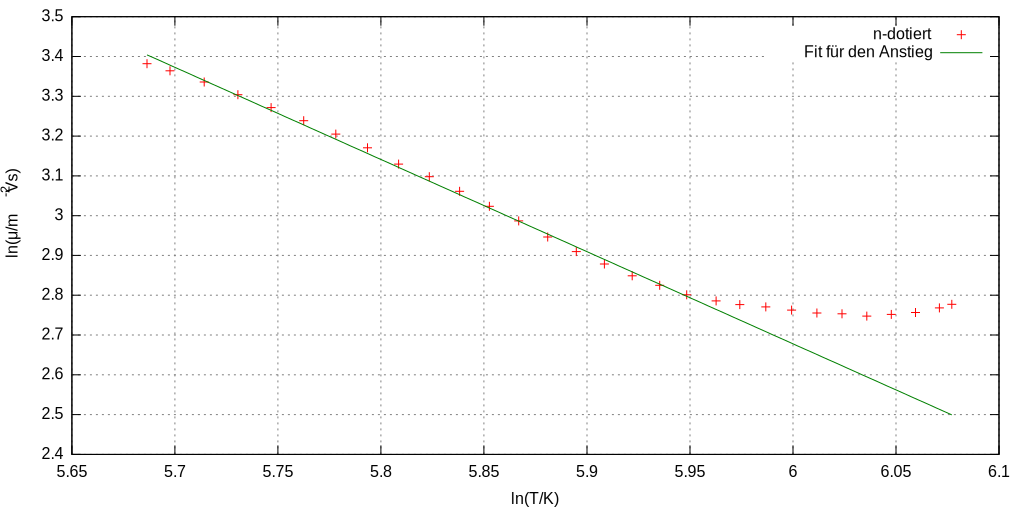
\includegraphics[width=\textwidth]{messwerte/beweglichkeitn.pdf}
	\caption{Logarithmus der Beweglichkeit $\mu\ix{n}$ als Funktion des Logartihmus der Temperatur} \label{img:mu-n}
\end{figure}
\begin{figure}[H]
	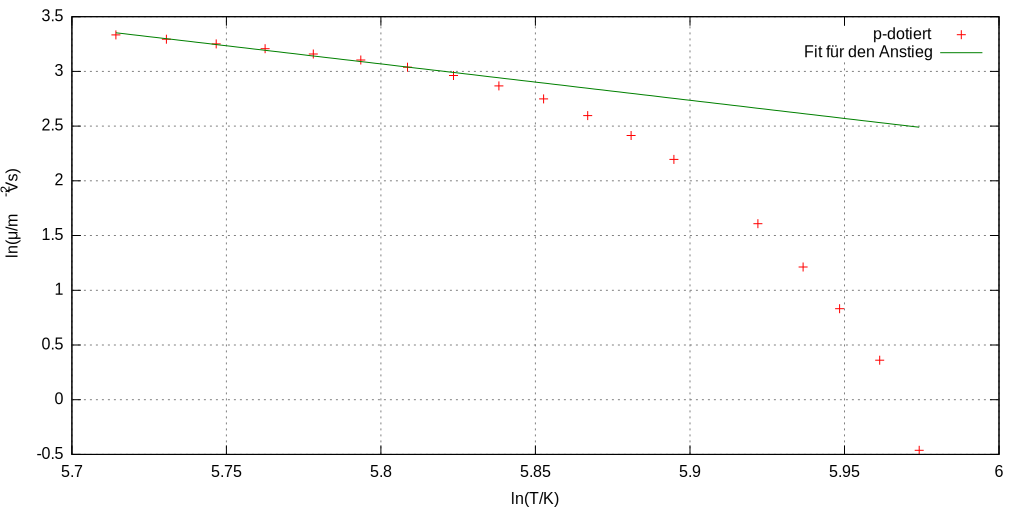
\includegraphics[width=\textwidth]{messwerte/beweglichkeitp.pdf}
	\caption{Logarithmus von $\mu\ix{p}$ über dem Logarithmus von $T$} \label{img:mu-p}
\end{figure}
\section{Quellen}
%\section{Anhang}
\end{document}